\subsubsection*{Informazioni sul package}
\begin{figure}[h]
	\centering
	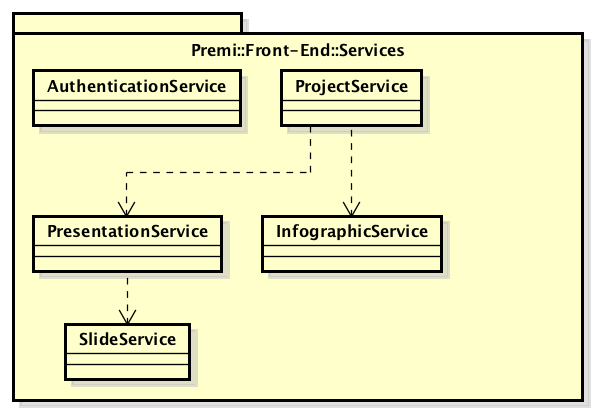
\includegraphics[width=0.9\linewidth]{img/front-end_services}
	\caption[Premi::Front-End::Services]{Premi::Front-End::Services}
\end{figure}
\begin{itemize}
	\item \textbf{Descrizione}: Il package contiene gli elementi per creare i service del \gls{front-end}, ovvero per creare gli oggetti che consentono di interfacciarsi con le API \gls{REST} del \gls{back-end}, popolare il model del client e richiedere l'esecuzione di altre operazioni necessarie al server;
	\item \textbf{Interazione con altri package}:
	\begin{itemize}
		\item Vi è un'interazione con il package Premi::Front-End::Model per raccogliere i dati da passare al back-end attraverso le opportune chiamate REST.
	\end{itemize}
\end{itemize}

\subsubsection*{Classi contenute}
\begin{itemize}

    \item Premi::Front-End::Services::AuthenticationService:
	\begin{itemize}
		\item \textbf{Descrizione}: classe per la gestione dell'autenticazione e della registrazione di un utente;
		\item \textbf{Relazioni con altre classi}:
		\begin{itemize}
			\item Premi::Front-End::Controllers::AuthenticationCtrl;
			\item Premi::Front-End::Model::User.
		\end{itemize}
	\end{itemize}

    \item Premi::Front-End::Services::ProjectService:
	\begin{itemize}
		\item \textbf{Descrizione}: classe per la gestione di un progetto e dei suoi componenti (presentazione e infografiche);
		\item \textbf{Relazioni con altre classi}:
		\begin{itemize}
			\item Premi::Front-End::Controllers::ProjectsController;
			\item Premi::Front-End::Controllers::ProjectController;
			\item Premi::Front-End::Model::Projects;
			\item Premi::Front-End::Model::Project.
		\end{itemize}
	\end{itemize}

    \item Premi::Front-End::Services::PresentationService:
	\begin{itemize}
		\item \textbf{Descrizione}: classe per la gestione di una presentazione e dei suoi dati;
		\item \textbf{Relazioni con altre classi}:
		\begin{itemize}
			\item Premi::Front-End::Controllers::PresentationController;
			\item Premi::Front-End::Controllers::PresentationEditorController;
			\item Premi::Front-End::Model::Presentation.
		\end{itemize}
	\end{itemize}

    \item Premi::Front-End::Services::SlideService:
	\begin{itemize}
		\item \textbf{Descrizione}: classe per la gestione di una slide, della sua modifica e degli elementi presenti in essa;
		\item \textbf{Relazioni con altre classi}:
		\begin{itemize}
			\item Premi::Front-End::Controllers::SlideEditorController;
			\item Premi::Front-End::Controllers::ComponentController;
			\item Premi::Front-End::Model::Slide.
		\end{itemize}
	\end{itemize}

    \item Premi::Front-End::Services::InfographicService:
	\begin{itemize}
		\item \textbf{Descrizione}: classe per la gestione di una infografica e della sua modifica;
		\item \textbf{Relazioni con altre classi}:
		\begin{itemize}
			\item Premi::Front-End::Controllers::InfographicEditorController;
			\item Premi::Front-End::Model::Infographic.
		\end{itemize}
	\end{itemize}

\end{itemize}
